\documentclass[11pt,letterpaper]{article}
\bibliographystyle{ieeetr}
\usepackage[backend=biber,style=numeric]{biblatex} 
\addbibresource{reference.bib} 
\usepackage[utf8]{inputenc}
\usepackage{graphicx}

\usepackage{fullpage}

\begin{document}


\title{Knowledge-CLIP for Limited Data: Enhancing Semantic Alignment in Small-Scale Datasets}


\author{
Zhanhao Liu (zhanhaol@umich.edu), 
Huanchen Jia (jhuanch@umich.edu),\\
Qiulin Fan (rynnefan@umich.edu),
Lingyu Meng (jmly@umich.edu)
}

\date{02/03/2025}


\maketitle


\section{Problem statement}
Multimodal representation learning, particularly through frameworks like Contrastive Language–Image Pretraining (CLIP), has shown significant promise in bridging the gap between textual and visual data. CLIP-based models excel in tasks such as zero-shot classification, cross-modal retrieval, and transfer learning by learning joint embeddings of text and images. However, the performance of these models is heavily reliant on the quality, diversity, and scale of the training data. Current multimodal datasets often suffer from issues such as biases, noise, imbalances, and limited diversity, which can hinder the generalization and robustness of CLIP-based systems. While much attention has been given to improving model architectures and training strategies, there is a critical need to explore data-centric methods—such as dataset curation, augmentation, debiasing, and sampling—to address these challenges. This research focuses on developing and evaluating data-centric approaches to enhance the effectiveness of CLIP-based multimodal representation learning, ultimately enabling more reliable and scalable models for real-world applications.\\
We aim to design data-centric augmentations to improve CLIP performance on small training datasets. Our current interest lies in adpting and improving the Knowledge-CLIP framework\cite{pan2022contrastivelanguageimagepretrainingknowledge} to small-sized datasets, and further create our own model based on it.



\section{Significance}
Contrastive Language–Image Pretraining (CLIP) has revolutionized multimodal representation learning by enabling models to learn joint embeddings of text and images through contrastive learning. While CLIP has shown remarkable performance in zero-shot and transfer learning tasks, its effectiveness is highly dependent on the quality, diversity, and scale of the training data. Existing multimodal datasets often contain biases, noise, and imbalances, which can hinder the generalization and robustness of CLIP-based models. Despite significant progress in model architectures and pretraining strategies, the role of data-centric methods—such as dataset curation, augmentation, debiasing, and sampling—remains underexplored. Addressing these data-related challenges is critical to unlocking the full potential of CLIP-based multimodal representation learning.



\section{Related work} 
CLIP (Contrastive Language-Image Pre-Training) is a multimodal representation learning model which leanrs to understand both text and image jointly by combining them in a shared embedding space. And its performance is shown recently that it could be enhanced by leverging the difficulty in training.\\
Currently the exisiting methods mostly improve in the following perspectives.\\
\begin{itemize}
    \item \textbf{Hard Negative Mining}: Hard negative examples are those that are semantically similar to the positive samples but belong to different classes, making it challenging for the model to distinguish between them. In contrastive learning, two primary strategies enhance model performance: generation-based methods and regularization-based methods. Generation-based methods, such as NegCLIP and SVLC, create hard negatives by altering positive samples to produce semantically similar yet incorrect pairs, challenging models to discern subtle differences. Regularization-based methods employ strategies like intra-modal contrastive loss and ranking cross-modal hard negatives to refine learning. These approaches adjust the training process to emphasize harder negatives, improving the model's discriminative capabilities.
    \item \textbf{Fine-Grained Cross-Modal Alignment Fine-Tuning}: Some previous works such as FILIP enhances multimodal alignment by matching local image patches with specific text tokens via a similarity matrix. Unlike CLIP’s global image-text matching, it computes token-level contrastive losses, forcing visual and textual tokens to mutually select their most relevant counterparts. The regional
    \item \textbf{Rewritw Empowered by Large Language Model}: Generate synthetic image-text pairs using diffusion models (e.g., Stable Diffusion) or text-to-image generators.
\end{itemize}


CLIP (Contrastive Language-Image Pre-Training) as a neural network trained on diverse image-text pairs, can predict relevant text for a given image using natural language instructions, showcasing zero-shot capabilities similar to GPT models. 
Notably, CLIP matches ResNet50's performance on ImageNet in a zero-shot setting without using labeled examples, highlighting its ability to generalize across tasks without task-specific training. 
In particular, there are recent studies that show that there is a positive correlation between CLIP performance and training objective difficulty. 
Yuksekgonul et al. (2022, \cite{yuksekgonul2023visionlanguagemodelsbehavelike}) demonstrated that models struggle with relation, attribution, and order understanding and the potential solution could be applying a modification on training procedure namely "composition-aware hard negative mining". 
Alternatively, there are also teams solving the problem in approach "constructing mini batches that include similarity clusters to increase the difficulty of negative examples". (Liu et al., n.d.). 
Besides the above, increasing data diversity through language rewriting has also shown the potential to improve the performance \cite{fan2023improvingcliptraininglanguage}.

Here are another three great references that we study together:\\
(1) Contrastive Language-Image Pre-Training with Knowledge Graphs:
\cite{pan2022contrastivelanguageimagepretrainingknowledge}
This paper introduces Knowledge-CLIP, an extension of the CLIP model that incorporates knowledge graphs. It motivates from the fact traditional vision-language pre-training methods, like CLIP, rely on large-scale image-text pairs but often miss fine-grained semantic relationships.
To improve it utilizes separate Transformer-based encoders for images and text to extract raw features. Leverages knowledge graphs to provide structured semantic relationships between entities (which can be images or text) and relations (described in language).
Employs a multi-modal Transformer encoder to fuse these features, enforcing a semantic alignment between modalities through knowledge-based objectives.  For Objective functions it included triplet-based loss and graph-based loss and a factor from result different original CLIP to cut down the training complexity.\\
(2) Unified Framework for Contrastive Language–Image Pre-training\cite{lee2022uniclipunifiedframeworkcontrastive}:
This approach further refines contrastive learning by introducing a unified space where both inter-domain and intra-domain contrastive losses are jointly optimized. Unlike prior methods that separate these losses into individual spaces, this unified framework ensures that all supervision signals are effectively combined, leading to more robust feature alignment. This is achieved through three major components: augmentation-aware feature embedding, MP-NCE loss, and domain-dependent similarity measures. These techniques collectively enhance the model’s ability to learn meaningful relationships between visual and textual data, resulting in improved performance across a diverse set of downstream tasks.\\
(3) CLIP the bias:  How Useful is Balancing Data in Multimodal Learning?\cite{alabdulmohsin2024clipbiasusefulbalancing}:
The essay investigates the role of data balancing in mitigating biases within contrastive language-image pretraining (CLIP) models, analyzing both its strengths and limitations. The study begins by reaffirming that CLIP models can inadvertently absorb societal stereotypes and explores how biases manifest in multimodal learning.To address these biases, the authors propose a novel algorithm called Multi-Modal Moment Matching (M4), which aims to reduce both representation and association biases by adjusting first- and second-order statistical properties of multimodal data. They conduct extensive experiments to examine how M4 interacts with various factors, such as model architecture\textbf{, }data representation, and dataset size.\\
This will be followed by more.

\section{Proposed Approach}
Knowledge-CLIP enhances CLIP's performance in semantic alignment and reasoning tasks by incorporating Knowledge Graphs (KGs), which enable the extraction of structural information between entities. Additionally, it leverages Knowledge Distillation (KD) Loss to distill knowledge from the original CLIP model, preventing catastrophic forgetting when adapting to new tasks.

Originally, Knowledge-CLIP was designed for large-scale datasets and heavily relies on a multimodal transformer architecture. However, we argue that its knowledge-driven semantic alignment capability can be effectively adapted to small-scale datasets. The \textbf{KG-enhanced learning} mechanism in Knowledge-CLIP provides several advantages:
\begin{itemize}
    \item Compensating for missing relational information in small datasets, mitigating the risk of overfitting to a limited data distribution.
    \item Improving the model’s ability to understand object attributes and relationships, thereby enhancing generalization.
\end{itemize}
Our goal is to modify Knowledge-CLIP to ensure its effectiveness on small datasets while retaining its knowledge-enhanced learning capabilities. Specifically, at this time as a draft, we plan to:
\begin{enumerate}
    \item Retain Knowledge-CLIP’s knowledge enhancement mechanism while\textbf{ removing its complex multimodal transformer structure} to reduce computational overhead.
    \item \textbf{Replace the heavy encoders with lightweight alternatives}:
    \begin{itemize}
        \item Image encoder: Replace ViT-Large with ViT-Small.
        \item Text encoder: Replace CLIP’s Transformer with \textbf{DistilBERT} or other lightweight models.
    \end{itemize}
    \item Incorporate more efficient optimization strategies, such as \textbf{SimCLIP}\cite{liu2024an} and \textbf{Adaptive Hard Negative Mining (AHNM)}, introducing a more lightweight contrastive learning optimization strategy.
    \item Freeze part of the model parameters, fine-tuning only the \textbf{top layers and projection head}, reducing overfitting risks associated with small datasets.
    \item Apply\textbf{ Low-Rank Adaptation (LoRA)} within Knowledge-CLIP’s multimodal module, adapting only a small subset of parameters for efficient training.
    \item \textbf{Introduce Fair Contrastive Loss (FCL)\cite{alabdulmohsin2024clipbiasusefulbalancing}} to prevent the model from learning spurious associations present in the dataset, thereby reducing Representation Bias.
\end{enumerate}

\subsection{Pipeline illustration}
\begin{center}
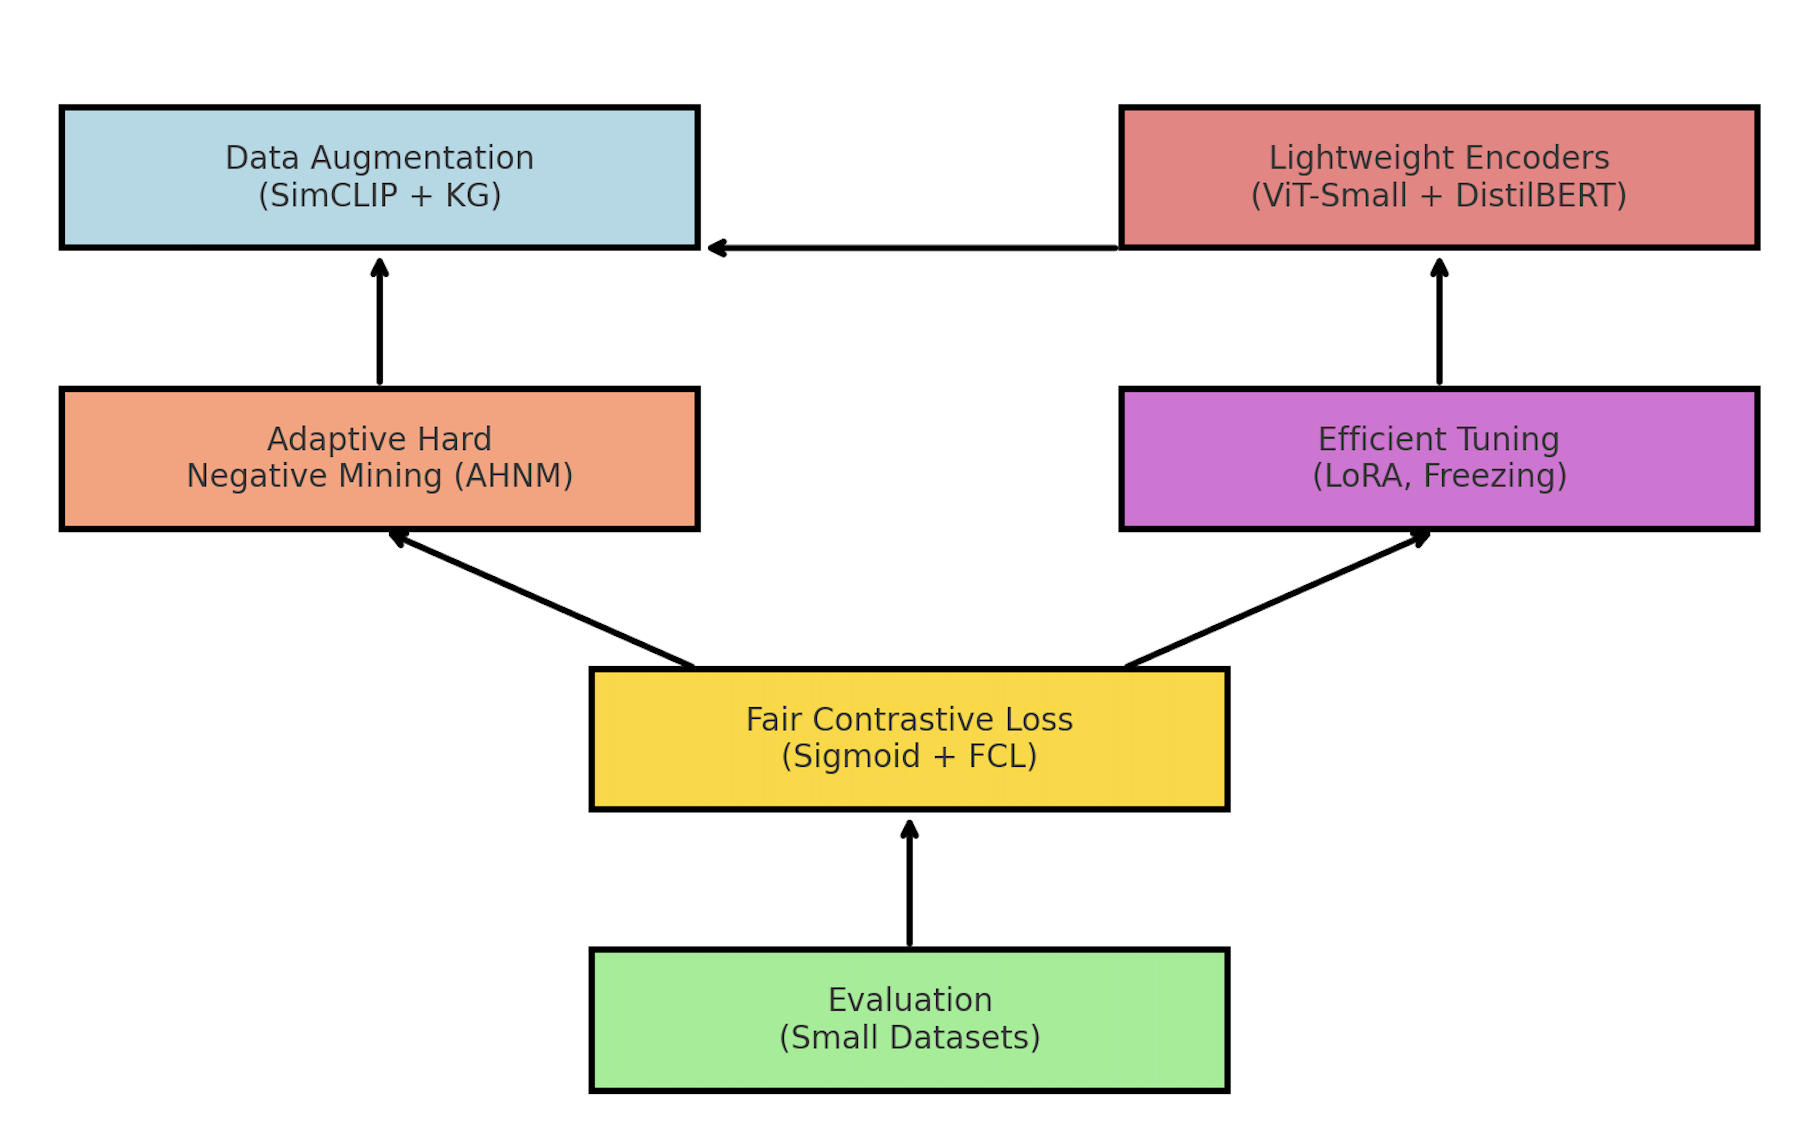
\includegraphics[width=12cm]{proposal/pipeline_draft.png}
    
\end{center}


\printbibliography
\end{document}